\begin{chapter}{Semiclassical Wavepackets}
\label{ch:wavepackets}

\section{Basis functions}

In this section we present a particular form of wavepackets defined
by G. Hagedorn, see for example \cite{H_semiclassical_i,H_semiclassical_iii}
and particularly \cite{H_ladder_operators}.

These wavepackets are a general class of orthonormal basis functions for an $L^2\ofs{\mathbb{R}^d}$
space. For the $d$ dimensional space they are defined as follows. Let $q \in \mathbbm{R}^d$
be the position and $p \in \mathbbm{R}^d$ the momentum vector of the package. Further
there are complex matrices $P, Q \in \mathbbm{C}^{d \times d}$ which obey the following
important relations

\begin{equation} \label{eq:symplecticity_condition}
\begin{split}
  Q\T P - P\T Q & = 0 \\
  Q\herm P - P\herm Q & = 2 i \id  \,.
\end{split}
\end{equation}

With these parameters we can now define the ground state wavefunction $\phi_0$
depending on arbitrary but fixed parameters as

\begin{equation} \label{eq:hagedorn_groundstate_dd}
\begin{split}
  \phi_0 \left[ P,Q,p,q \right] \ofs{x}
  \assign &
  \left(\pi\varepsilon^2\right)^{-\frac{d}{4}} \det\left(Q\right)^{-\frac{1}{2}} \\
  & \cdot \exp \left(
      \frac{i}{2\varepsilon^2} \dotp{\left(x-q\right)}{PQ^{-1}\left(x-q\right)}
      + \frac{i}{\varepsilon^2} \dotp{p}{\left(x-q\right)}
  \right)
\end{split}
\end{equation}

where $x \in \mathbb{R}^d$. Also $\varepsilon$ enters this equation with a constant
numerical value during all computations\footnote{
In contrast to some other authors we use the notation of $P \assign iB$ and $Q \assign A$
and $q \assign a$ for the position and $p \assign \eta$ for the momentum. The motivation
for this change are the equations of motion of $P$ and $Q$ that become the
classical equations.}.

The eigenfunctions of the harmonic oscillator are contained as special cases
in the more general formulae for these wavepackets.

For the semiclassical wavepackets we can define and use ladder operators in the
same manner as one does for the harmonic oscillator. This analogy builds on the fact that
these wavepackets diagonalize the general quadratic Hamiltonian. Before we define
these operators, let's restrict the dimension of the position space to one. This
way we can avoid some difficulties that have no relevance for us now.

\subsection{Restriction to one space dimension}

The restriction to one space dimension where $d=1$ simplifies things a lot because
the vectors $p$ and $q$ and especially the matrices $P$ and $Q$ all reduce to scalar
values. Further we don't need to bother with multi-index notation for $k$.

First we simplify the ground state \eqref{eq:hagedorn_groundstate_dd} to the one
dimensional case

\begin{equation} \label{eq:hagedorn_groundstate_1d}
  \phi_0 \left[ P,Q,p,q \right] \ofs{x}
  \assign
  \left(\pi\varepsilon^2\right)^{-\frac{1}{4}} Q^{-\frac{1}{2}}
  \exp \left(
      \frac{i}{2\varepsilon^2} PQ^{-1}\left(x-q\right)^2
      + \frac{i}{\varepsilon^2} p\left(x-q\right)
  \right) \,.
\end{equation}

\subsection{Ladder operators}

Now let's take a closer look at the ladder operators from reference \cite{H_ladder_operators}.
As mentioned above there exists a lowering operator $\mathcal{L}$ and a raising
operator $\mathcal{R}$ for semiclassical wavepackets. We will use these ladder
operators later for defining the wavefunctions $\phi_k$ of higher states $k \geq 1$.
The ladder operators are defined as

\begin{equation} \label{eq:definition_ladder_ops}
\begin{split}
  \mathcal{R} &= \frac{i}{\sqrt{2 \varepsilon^2}} \left( \conj{P} \left(x-q\right) - \conj{Q} \left(y-p\right) \right) \\
  \mathcal{L} &= - \frac{i}{\sqrt{2 \varepsilon^2}} \left( P \left(x-q\right) - Q \left(y-p\right) \right)
\end{split}
\end{equation}

where $y \assign -i \varepsilon^2 \nabla$. It exists a lowest state which can not
be lowered further by $\mathcal{L}$. This state is the zero state and acts as the
bottom of this ladder

\begin{equation} \label{eq:ladder_ops_base}
  \mathcal{L} \phi_0 = 0 \,.
\end{equation}

On the other hand we can apply the raising operator to the ground state and create $\phi_1$

\begin{equation} \label{eq:ladder_ops_phi_0}
  \phi_1 = \mathcal{R} \phi_0 \,.
\end{equation}

In the same way we can create $\phi_k$ for arbitrary $k$ by applying $\mathcal{R}$
multiple times. To be more concrete, the following formulae bring the different
states into relation

\begin{equation} \label{eq:applied_ladder_ops}
\begin{split}
  \phi_{k+1} & = \frac{1}{\sqrt{k+1}} \mathcal{R} \phi_k \\
  \phi_{k-1} & = \frac{1}{\sqrt{k}} \mathcal{L} \phi_k \,.
\end{split}
\end{equation}

To get the state $\phi_k$ from the given $\phi_0$ we have to let $\mathcal{R}$ act $k$
times. Together with the prefactors this yields

\begin{equation}
  \phi_k \assign \frac{1}{\sqrt{k!}} \mathcal{R}^k \phi_0 \,.
\end{equation}

Finally we can give an analytical closed form for the function $\phi_k$

\begin{multline} \label{eq:hagedorn_kstate_1d}
  \phi_k \left[ P,Q,p,q \right] \ofs{x}
  \assign
  2^{-\frac{k}{2}}\left(k!\right)^{-\frac{1}{2}}\left(\pi\varepsilon^2\right)^{-\frac{1}{4}} Q^{-\frac{k+1}{2}}\conj{Q}^{\frac{k}{2}}
  \cdot H_k\ofs{\varepsilon^{-1}\left|Q\right|^{-1}\left(x-q\right)} \\
  \cdot \exp \left(\frac{i}{2\varepsilon^2} PQ^{-1}\left(x-q\right)^2 + \frac{i}{\varepsilon^2} p\left(x-q\right) \right)
\end{multline}

where $H_k\ofs{\xi}$ is the Hermite polynomial \footnote{
We use the following definition for the Hermite polynomials
\begin{equation}
  H_k\ofs{\xi} \assign \left(-1\right)^k e^{\xi^2} \left( \frac{\partial}{\partial\xi} \right)^k e^{-\xi^2}
\end{equation}}
of degree $k$. For an arbitrary but fixed $\varepsilon > 0$ and fixed parameters $P$,
$Q$ and given position $q$ and momentum $p$ these functions $\phi_k$ build a complete
basis set $\{\phi_k\}_{k=0}^\infty$ of the space $L^2$. This infinite basis can be
truncated at some upper value $K \gg 0$ and we get the set $\{\phi_k\}_{k=0}^K$
of functions. This will be used as basis for the semiclassical wavepackets later on.

To end this section, let's emphasize again the close relationship to the eigenfunctions
of the harmonic oscillator. Suppose $P=i$, $Q=1$, choose the origin as position and assume
the wavepacket has no momentum, thus $p=q=0$. Further, assume $\varepsilon = 1$.
If we now plug these values in \eqref{eq:hagedorn_kstate_1d} we get

\begin{equation}
  \Ket{\varphi_k} = \frac{H_k\ofs{x} e^{-\frac{x^2}{2}}}{\pi^{\frac{1}{4}}2^{\frac{k}{2}}\sqrt{k!}}
\end{equation}

which is exactly the well known expression for the harmonic oscillator.


\section{Definition of scalar wavepackets}

After we have defined a basis set $\{\phi_0, \phi_1, \ldots\}$ for the infinite
dimensional Hilbert space of states we can now define the exact form of a state
$\Ket{\Phi}$. Each state is represented by a linear combination of the basis
functions $\phi_k$. Of course the single basis functions are valid states too.

Assume we truncate the Hilbert space and use finite many basis functions. Let
$K$ be the maximal number of basis functions. Further let $S \in \mathbb{C}$ be
a global phase. Any scalar wavepacket can now be written as

\begin{equation} \label{eq:hawp_def_single}
  \Ket{\Phi\of{x}} \assign e^{\frac{iS}{\varepsilon^2}} \sum_{k=0}^{K-1} c_k \phi_k \of{x}
\end{equation}

where $c_k \in \mathbb{C}$ are the coefficients of this linear combination. We can
collect them in a vector $c \assign \left(c_0, \ldots, c_{K-1}\right)\T$. For later
reference, we call the set

\begin{equation} \label{eq:hagedorn_parameters}
  \Pi \assign \{P, Q, S, p, q\}
\end{equation}

of variables the \emph{Hagedorn parameters} of a scalar wavepacket $\Ket{\Phi}$
of form \eqref{eq:hawp_def_single}. This set includes the four parameters
$P$, $Q$, $p$ and $q$ that come from the basis functions $\phi_k$ given by
equation \eqref{eq:hagedorn_kstate_1d} as well as the global phase
\footnote{Depending on the context, the global phase $S$ may or may not be
part of the set denoted by $\Pi$.}
that enters the above linear combination. These values play an important role in
the wavepacket based algorithms discussed in \cite{FGL_semiclassical_dynamics}.

\begin{figure}
  \centering
  \subfloat[][]{
    \label{fig:hawp_impulse_0_0}
    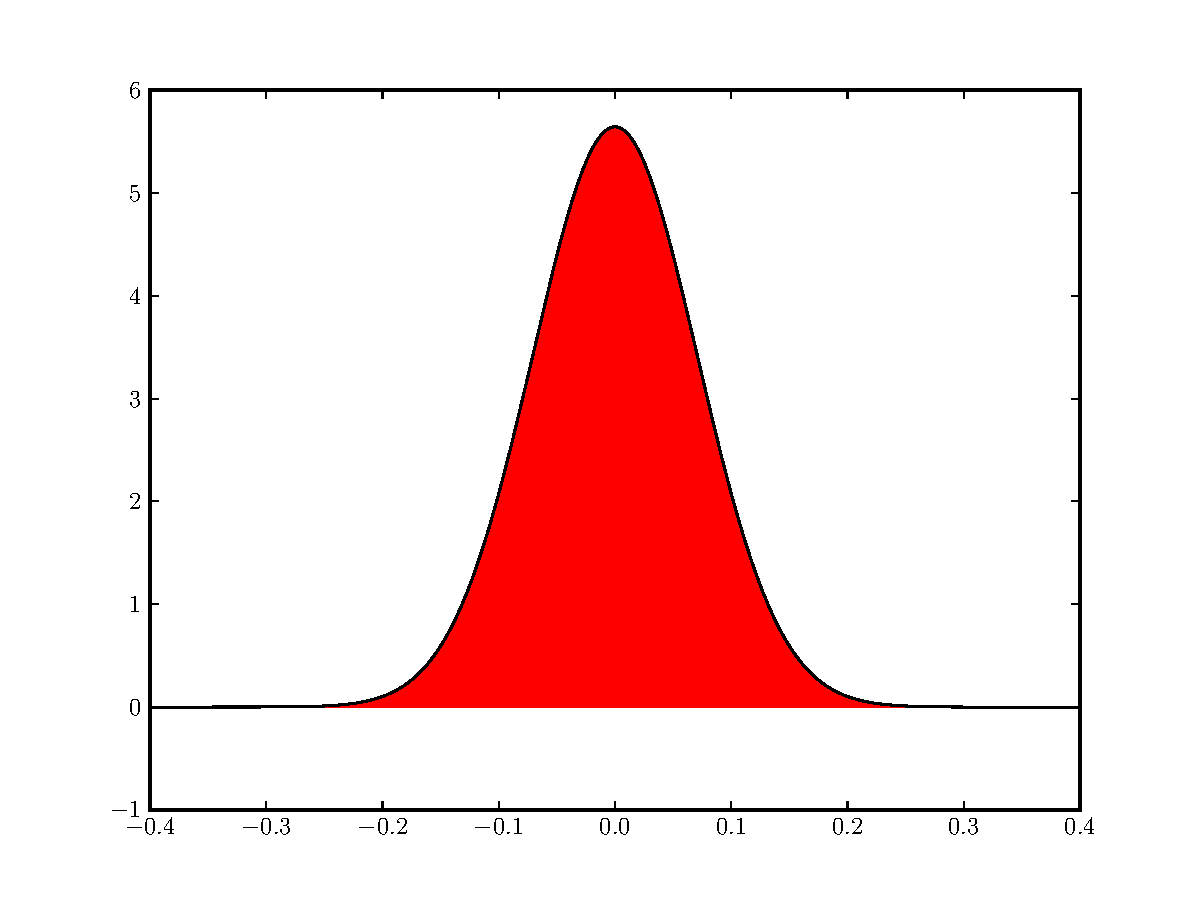
\includegraphics[width=0.5\linewidth]{./figures/hagedorn_wp_impulse_0_0.pdf}
  }
  \subfloat[][]{
    \label{fig:hawp_impulse_0_25}
    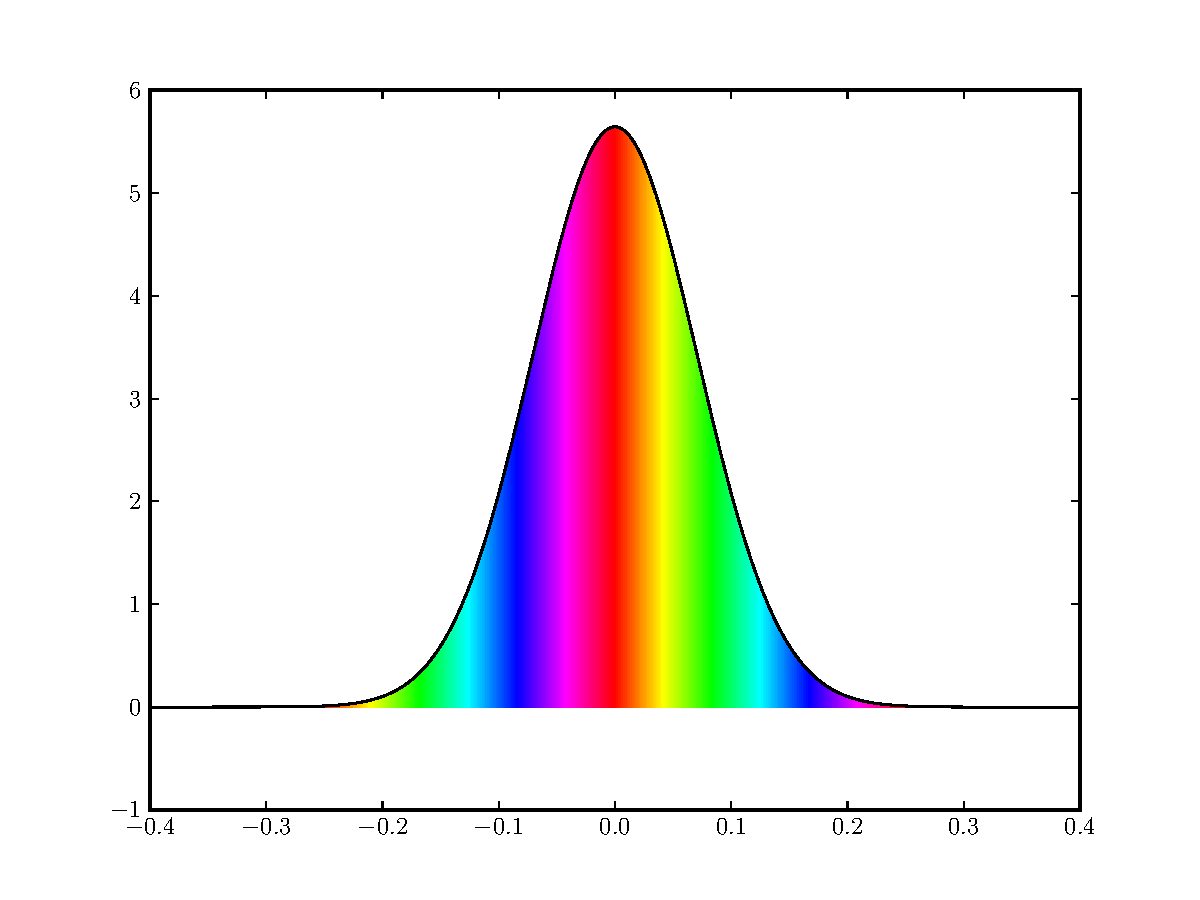
\includegraphics[width=0.5\linewidth]{./figures/hagedorn_wp_impulse_0_25.pdf}
  } \\
  \subfloat[][]{
    \label{fig:hawp_impulse_0_5}
    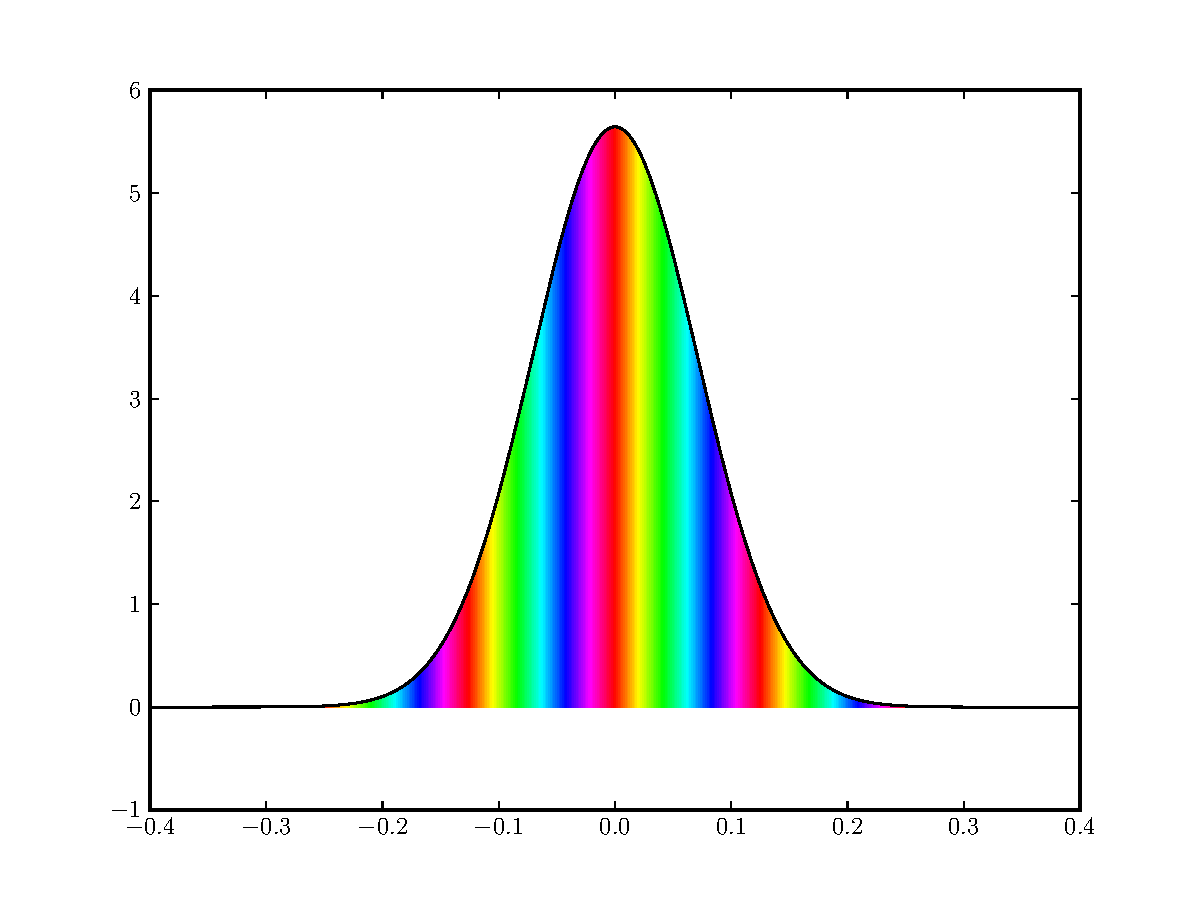
\includegraphics[width=0.5\linewidth]{./figures/hagedorn_wp_impulse_0_5.pdf}
  }
  \subfloat[][]{
    \label{fig:hawp_impulse_1_0}
    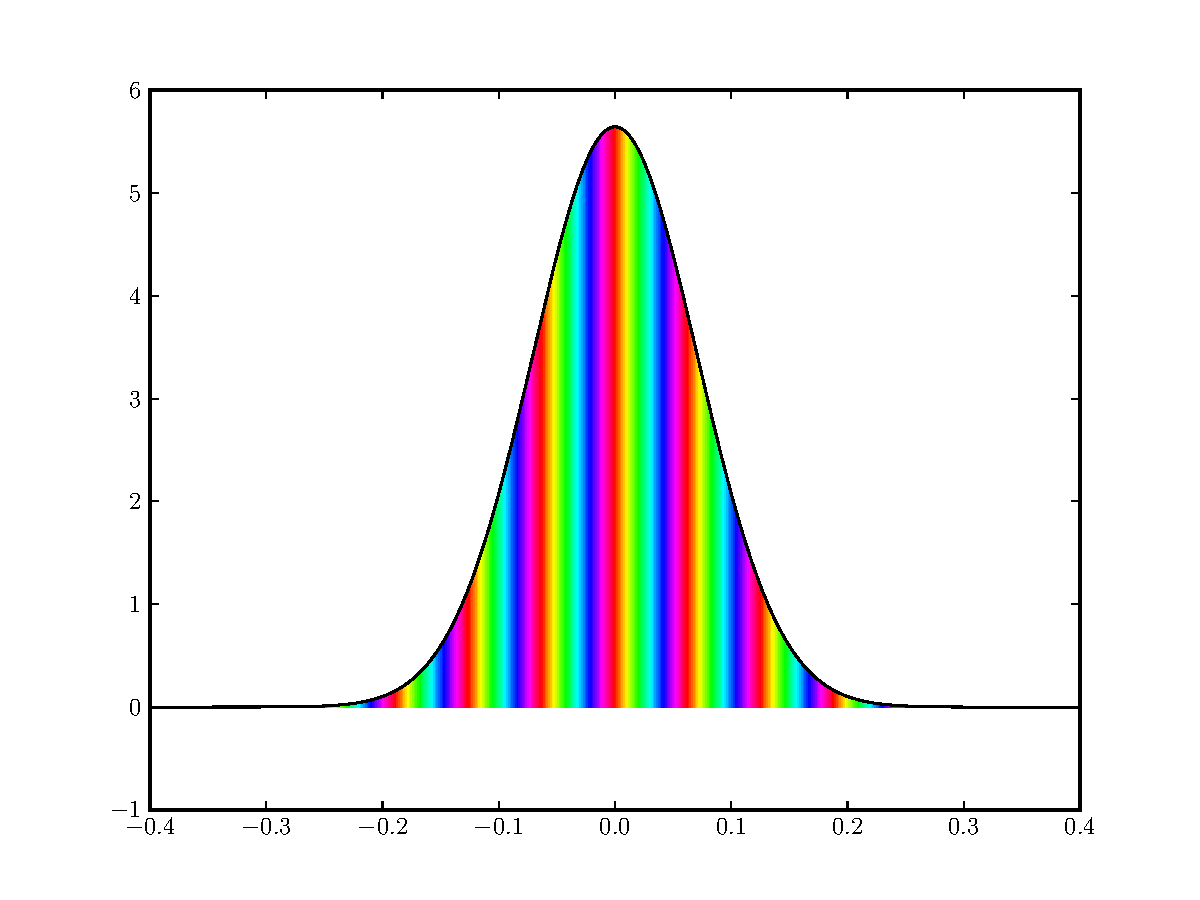
\includegraphics[width=0.5\linewidth]{./figures/hagedorn_wp_impulse_1_0.pdf}
  } \\
  \subfloat[][]{
    \label{fig:hawp_impulse_1_5}
    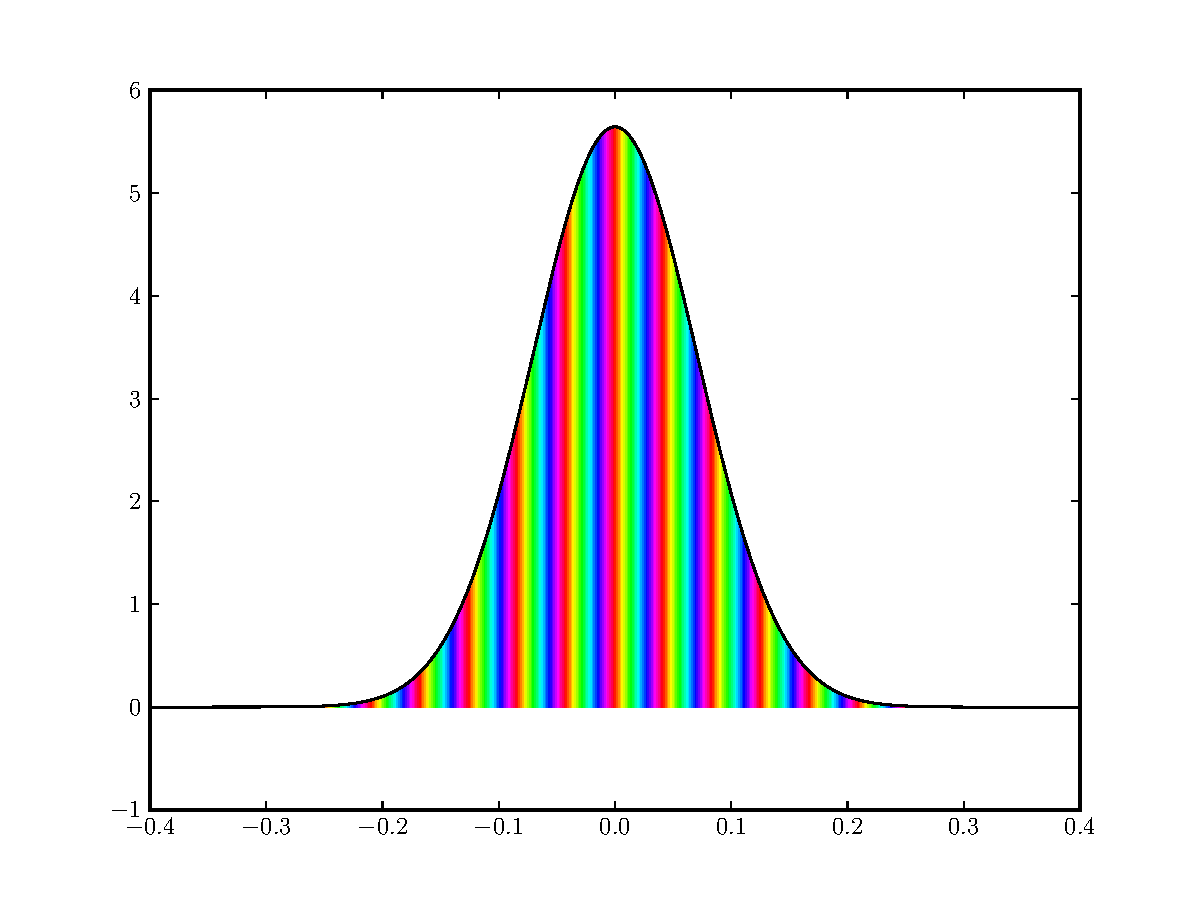
\includegraphics[width=0.5\linewidth]{./figures/hagedorn_wp_impulse_1_5.pdf}
  }
  \subfloat[][]{
    \label{fig:hawp_impulse_2_0}
    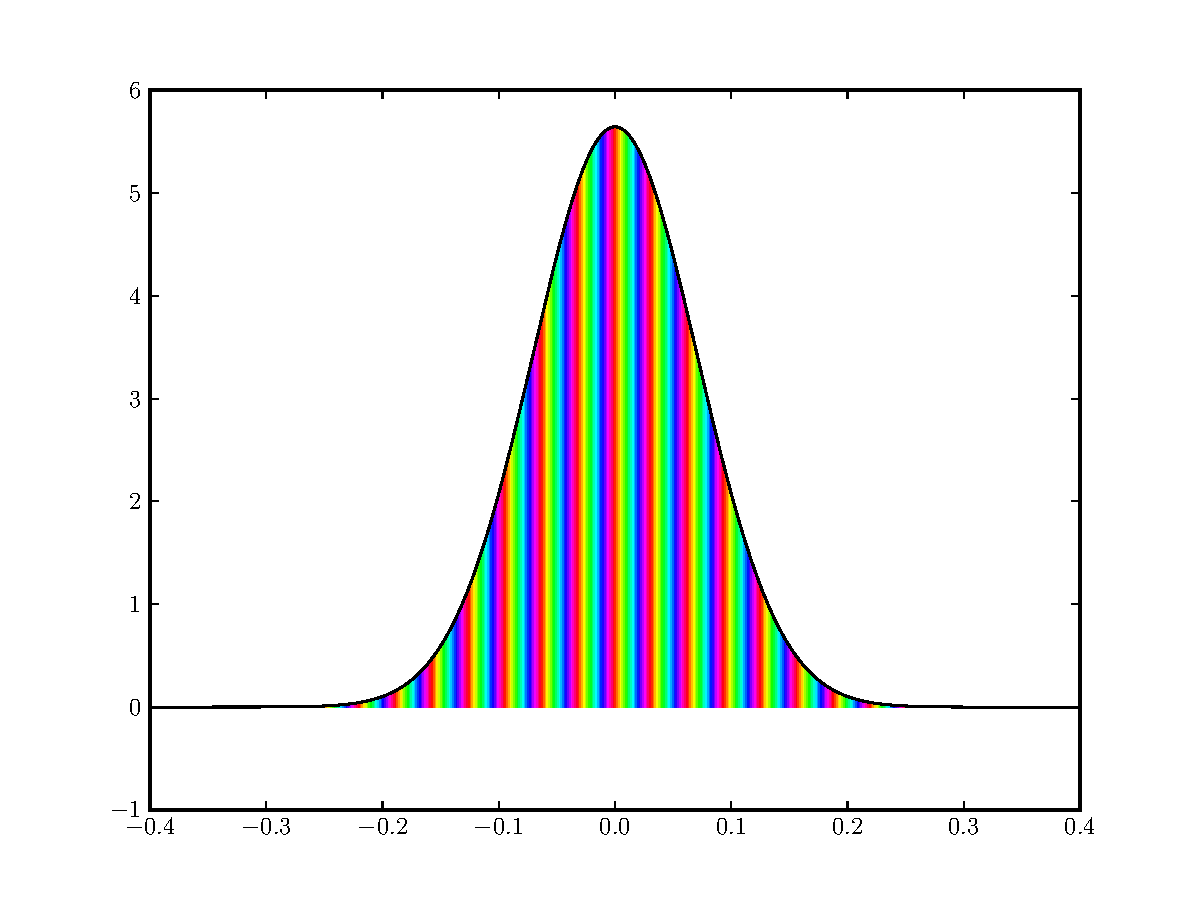
\includegraphics[width=0.5\linewidth]{./figures/hagedorn_wp_impulse_2_0.pdf}
  }
  \caption[Hagedorn wavepackets $\Ket{\Psi}$ with increasing momentum]{
    Hagedorn wavepackets $\Ket{\Psi}$ with increasing momentum. The plots show the
    absolute value $\Braket{\Psi|\Psi}$ and the local phase. The other parameters
    are $\varepsilon = 0.1$ and $P=i$, $Q=1$ and $S=0$.
    \subref{fig:hawp_impulse_0_0}  $q = 0.0$ and $p = 0.0$
    \subref{fig:hawp_impulse_0_25} $q = 0.0$ and $p = 0.25$
    \subref{fig:hawp_impulse_0_5}  $q = 0.0$ and $p = 0.5$
    \subref{fig:hawp_impulse_1_0}  $q = 0.0$ and $p = 1.0$
    \subref{fig:hawp_impulse_1_5}  $q = 0.0$ and $p = 1.5$
	\subref{fig:hawp_impulse_2_0}  $q = 0.0$ and $p = 2.0$
    \label{fig:hawp_impulse}
  }
\end{figure}


\section{Homogeneous vector valued wavepackets}

For the quantum dynamics with semiclassical wavepackets in the case of the vector
valued Schrödinger equation as defined by formula \eqref{eq:basics_tdse_vector} we
need a wavepacket $\Ket{\Psi}$ that is vector valued as well. Such a packet
$\Ket{\Psi}$ can be build as a vector of multiple scalar semiclassical packets.
Assume that the Hamiltonian $H$ in \eqref{eq:basics_tdse_vector} is a $N \times N$
matrix, thus there are $N$ energy levels and $\Ket{\Psi}$ needs to have $N$ components
too. Formally we define

\begin{align} \label{eq:hawp_def_state_vector}
  \Ket{\Psi} & \assign \Ket{ \begin{pmatrix}
                         \Phi_0\of{x} \\
                         \vdots \\
                         \Phi_{N-1}\of{x} \\
                       \end{pmatrix}}
\end{align}

where each of the $\Phi_i$ is of the form defined in \eqref{eq:hawp_def_single}.

All $\Phi_i$ share the same parameters $P$, $Q$, global phase $S$, average momentum
$q$ and average position $p$. We will call a wavepacket that fulfills this condition a \emph{homogeneous wavepacket}.
Equivalently we can say the only thing that differs between the $\Phi_i$ is the vector of coefficients $c$.
Therefore we add an index $i$ to the notation, $c^i$ stands for the coefficient vector of the component $\Phi_i$.
Thus a semiclassical wavepacket suitable for solving \eqref{eq:basics_tdse_vector}
has the important property that it is fully characterized by a single set $\Pi$ of
parameters $P$, $Q$, $S$, $p$ and $q$ and a vector $c^i$ of coefficients for each
component $\Phi_i$.


\section{Inhomogeneous vector valued wavepackets}

For advanced applications we may extend the definition \eqref{eq:hawp_def_state_vector}
of a state $\Ket{\Psi}$ and release the main restriction. In contrast to the homogeneous
wavepackets of the last section we allow that each component $\Phi_i$ has it's very
own set of parameters $P$, $Q$, $S$, $p$ and $q$. We call such a wavepacket an
\emph{inhomogeneous wavepacket}. To be able to distinguish the different variables
an index $i$ is added also to the parameters $\Pi$. Thus a wavepacket is fully
characterized by a set $\Pi_i$ of parameters $P_i$, $Q_i$, $S_i$, $p_i$ and $q_i$
and a vector $c^i$ of coefficients for each component $\Phi_i$.


\section{Numerical evaluation}

\subsection{Numerical evaluation of basis functions}

For the numerical simulation we will need to evaluate the functions $\phi_k\ofs{x}$
at some discrete grid nodes $x_i$. This seems to be a trivial task as we have a
closed form expression for $\phi_k$ given by equation \eqref{eq:hagedorn_kstate_1d}.
Although there is this expression for all $k$ it's a bad idea to use it directly.
One critical point in this formula is the factorial. It will soon result in a
numerical overflow even for relatively small $k$. Therefore we need a better approach.
An idea is to evaluate the ground state and recursively calculate the higher states
based on these values. The essential three term recursion can be obtained as follows.
We start with the function for $\phi_0$ which we can evaluate numerically without
much troubles. It is just a Gaussian exponential. (Note that we omit a factor of
$Q^{-\frac{1}{2}}$ for the moment.)

Applying the raising operator $\mathcal{R}$ once results in

\begin{equation}
  \phi_1\ofs{x} = Q^{-1} \sqrt{\frac{2}{\varepsilon^2}}\left(x-q\right) \cdot \phi_0
\end{equation}

and for the general case we get the following three term recursion by applying
$\mathcal{R}$ on $\phi_k$ and rearranging the terms

\begin{equation} \label{eq:hagedorn_recursion_rel}
  \phi_{k+1}\ofs{x} = \sqrt{\frac{2}{\varepsilon^2}} \frac{1}{\sqrt{k+1}} Q^{-1}
                      \left(x-q\right) \phi_k\ofs{x}
                      - \sqrt{\frac{k}{k+1}} Q^{-1} \conj{Q} \phi_{k-1} \ofs{x} \,.
\end{equation}

This is exactly how the calculation is implemented in an efficient and numerically
stable way. Because later we will need the values for all $\phi_k$ from $k=0$
up to a maximum $k_{\text{max}}\rassign K$, it's not a disadvantage but rather a big benefit
that we have to evaluate all previous functions for any $\phi_k$.

\begin{algorithm}
\caption{Evaluate basis functions $\phi_k\ofs{x}$ of semiclassical wavepackets}
\label{al:evaluate_basis_functions}
\begin{algorithmic}
  \REQUIRE A set of grid or quadrature nodes $x$
  \REQUIRE A set $\Pi \assign \{P,Q,p,q\}$ of parameters
  \STATE // Base cases
  \STATE $\beta_0 \assign \pi^{-\frac{1}{4}} \varepsilon^{-\frac{1}{2}}
               \cdot \exp\left( \frac{i}{\varepsilon^2} \left(\frac{1}{2} P Q^{-1}
                               \left( x - q \right)^2
                               + p \left( x - q \right) \right)
                        \right)$
  \STATE $\beta_1 \assign Q^{-1} \sqrt{\frac{2}{\varepsilon^2}} \left(x-q\right) \cdot \beta_0$
  \STATE // Inductive steps
  \FOR{$k \assign 2$ \TO $K-1$}
    \STATE $\beta_k \assign Q^{-1} \sqrt{\frac{2}{\varepsilon^2}} \frac{1}{\sqrt{k}}
                         \cdot \left(x-q\right) \cdot \beta_{k-1}
                         - Q^{-1} \conj{Q} \sqrt{\frac{k-1}{k}} \cdot \beta_{k-2}$
  \ENDFOR
  \RETURN $B \assign \left(\beta_0, \ldots, \beta_{K-1}\right)\T$
\end{algorithmic}
\end{algorithm}

In praxis we do not call algorithm \ref{al:evaluate_basis_functions} for each grid
node $x_i \in \Gamma$ but use vectorization and calculate $B$ for all nodes
simultaneously so the returned $B$ is a two-dimensional matrix array.

\subsection{Numerical evaluation of wavepackets}

The numerical evaluation of a wavepacket $\Ket{\Psi}$ on given grid nodes $x_i$
is not difficult. We just evaluate all the basis functions $\phi_k$ and assemble the parts.
If we have an homogeneous wavepacket we can do this once and use these values
for all $N$ components of $\Ket{\Psi}$. Otherwise we have to evaluate the basis
functions individually for each component $n$ of an inhomogeneous wavepacket as
the basis functions differ by their Hagedorn parameters $\Pi$. Then we multiply
these values with the coefficients $c^n$ for each component. Finally we have to
multiply with the global phase exponential $e^{\left(\frac{i S}{\varepsilon^2}\right)}$.
For an inhomogeneous wavepacket we have to keep in mind that each component $n$
has its own phase $S_n$. The algorithm \ref{al:evaluate_wave_packets_on_grid}
shows this procedure in the most general form. The outer for loop iterates over
all components of $\Ket{\Psi}$ while the inner loop is responsible for evaluating
the basis functions $\phi_k^n$ with $\Pi^n$ given per component $n$. This part can
be implemented efficiently according to algorithm \ref{al:evaluate_basis_functions}.

\begin{algorithm}
\caption{Evaluate a vector valued wavepacket $\Ket{\Psi}$ on a set of nodes}
\label{al:evaluate_wave_packets_on_grid}
\begin{algorithmic}
  \REQUIRE A set of grid or quadrature nodes $x$
  \REQUIRE An arbitrary (in)homogeneous wavepacket $\Psi$
  \STATE // Iterate over all components of $\Ket{\Psi}$
  \FOR{$n = 0$ \TO $N-1$}
    \STATE given $\Pi_n$ as $\{P_n,Q_n,S_n,p_n,q_n\}$
    \STATE // Evaluate the basis for component $n$
    \FOR{$k=0$ \TO $K-1$}
      \STATE $\beta_k \assign \phi_k \left[P_n, Q_n, p_n, q_n\right] \ofs{x}$
    \ENDFOR
    \STATE // Calculate the exponential of the phase
    \STATE $\pi_n \assign \exp\ofs{\frac{i S_n}{\varepsilon^2}}$
    \STATE // Assemble the component $\Phi_n$
    \STATE $\Phi_n \assign \pi_n \cdot \sum_{k=0}^{K-1} c^n_k \beta_k$
  \ENDFOR
  \RETURN $\left(\Phi_0, \ldots, \Phi_{N-1}\right)\T$
\end{algorithmic}
\end{algorithm}

In the evaluation of the basis functions above we leave out a factor of
$\frac{1}{\sqrt{Q}}$ that will cancel with a $Q$ from the quadrature rule
in \eqref{eq:homogeneous_quadrature_rule} later.

\end{chapter}
